%%%%%%%%%%%%%%%%%%%%%%%%%%%%%%%%%%%%%%%%
% datoteka diploma-vzorec.tex
%
% vzorčna datoteka za pisanje diplomskega dela v formatu LaTeX
% na UL Fakulteti za računalništvo in informatiko
%
% vkup spravil Gašper Fijavž, december 2010
% 
%
%
% verzija 12. februar 2014 (besedilo teme, seznam kratic, popravki Gašper Fijavž)
% verzija 10. marec 2014 (redakcijski popravki Zoran Bosnić)
% verzija 11. marec 2014 (redakcijski popravki Gašper Fijavž)
% verzija 15. april 2014 (pdf/a 1b compliance, not really - just claiming, Damjan Cvetan, Gašper Fijavž)
% verzija 23. april 2014 (privzeto cc licenca)
% verzija 16. september 2014 (odmiki strain od roba)
% verzija 28. oktober 2014 (odstranil vpisno številko)
% verija 5. februar 2015 (Literatura v kazalu, online literatura)
% verzija 25. september 2015 (angl. naslov v izjavi o avtorstvu)
% verzija 26. februar 2016 (UL izjava o avtorstvu)
% verzija 16. april 2016 (odstranjena izjava o avtorstvu)
% verzija 5. junij 2016 (Franc Solina dodal vrstice, ki jih je označil s svojim imenom)


\documentclass[a4paper, 12pt]{book}
%\documentclass[a4paper, 12pt, draft]{book}  Nalogo preverite tudi z opcijo draft, ki vam bo pokazala, katere vrstice so predolge!
\def\onlycontent{tru} % comment out to show also the cover pages



\usepackage[utf8x]{inputenc}   % omogoča uporabo slovenskih črk kodiranih v formatu UTF-8
\usepackage[slovene,english]{babel}    % naloži, med drugim, slovenske delilne vzorce
\usepackage[pdftex]{graphicx}  % omogoča vlaganje slik različnih formatov
\usepackage{fancyhdr}          % poskrbi, na primer, za glave strani
\usepackage{amssymb}           % dodatni simboli
\usepackage{amsmath}           % eqref, npr.
%\usepackage{hyperxmp}
\usepackage[hyphens]{url}  % dodal Solina
\usepackage{comment}       % dodal Solina

\usepackage[pdftex, colorlinks=true,
						citecolor=black, filecolor=black, 
						linkcolor=black, urlcolor=black,
						pagebackref=false, 
						pdfproducer={LaTeX}, pdfcreator={LaTeX}, hidelinks]{hyperref}

\usepackage{color}       % dodal Solina
\usepackage{soul}       % dodal Solina
\usepackage[numbers]{natbib}  % dodal Solina

\usepackage{amsthm}
\usepackage{svg}

%%%%%%%%%%%%%%%%%%%%%%%%%%%%%%%%%%%%%%%%
%	DIPLOMA INFO
%%%%%%%%%%%%%%%%%%%%%%%%%%%%%%%%%%%%%%%%
\newcommand{\ttitle}{Digitalna topologija na grafih}
\newcommand{\ttitleEn}{Digital topology on graphs}
\newcommand{\tsubject}{\ttitle}
\newcommand{\tsubjectEn}{\ttitleEn}
\newcommand{\tauthor}{Jakob Drusany}
\newcommand{\tkeywords}{računalnik, računalnik, računalnik}
\newcommand{\tkeywordsEn}{computer, computer, computer}


%%%%%%%%%%%%%%%%%%%%%%%%%%%%%%%%%%%%%%%%
%	HYPERREF SETUP
%%%%%%%%%%%%%%%%%%%%%%%%%%%%%%%%%%%%%%%%
\hypersetup{pdftitle={\ttitle}}
\hypersetup{pdfsubject=\ttitleEn}
\hypersetup{pdfauthor={\tauthor, matjaz.kralj@fri.uni-lj.si}}
\hypersetup{pdfkeywords=\tkeywordsEn}


 


%%%%%%%%%%%%%%%%%%%%%%%%%%%%%%%%%%%%%%%%
% postavitev strani
%%%%%%%%%%%%%%%%%%%%%%%%%%%%%%%%%%%%%%%%  

\addtolength{\marginparwidth}{-20pt} % robovi za tisk
\addtolength{\oddsidemargin}{40pt}
\addtolength{\evensidemargin}{-40pt}

\renewcommand{\baselinestretch}{1.3} % ustrezen razmik med vrsticami
\setlength{\headheight}{15pt}        % potreben prostor na vrhu
\renewcommand{\chaptermark}[1]%
{\markboth{\MakeUppercase{\thechapter.\ #1}}{}} \renewcommand{\sectionmark}[1]%
{\markright{\MakeUppercase{\thesection.\ #1}}} \renewcommand{\headrulewidth}{0.5pt} \renewcommand{\footrulewidth}{0pt}
\fancyhf{}
\fancyhead[LE,RO]{\sl \thepage} 
%\fancyhead[LO]{\sl \rightmark} \fancyhead[RE]{\sl \leftmark}
\fancyhead[RE]{\sc \tauthor}              % dodal Solina
\fancyhead[LO]{\sc Diplomska naloga}     % dodal Solina


\newcommand{\BibTeX}{{\sc Bib}\TeX}

%%%%%%%%%%%%%%%%%%%%%%%%%%%%%%%%%%%%%%%%
% naslovi
%%%%%%%%%%%%%%%%%%%%%%%%%%%%%%%%%%%%%%%%  


\newcommand{\autfont}{\Large}
\newcommand{\titfont}{\LARGE\bf}
\newcommand{\clearemptydoublepage}{\newpage{\pagestyle{empty}\cleardoublepage}}
\setcounter{tocdepth}{1}	      % globina kazala

%%%%%%%%%%%%%%%%%%%%%%%%%%%%%%%%%%%%%%%%
% konstrukti
%%%%%%%%%%%%%%%%%%%%%%%%%%%%%%%%%%%%%%%%  
\newtheorem{izrek}{Izrek}[chapter]
\newtheorem{trditev}{Trditev}[izrek]
\newenvironment{dokaz}{\emph{Dokaz.}\ }{\hspace{\fill}{$\Box$}}

%%%%%%%%%%%%%%%%%%%%%%%%%%%%%%%%%%%%%%%%%%%%%%%%%%%%%%%%%%%%%%%%%%%%%%%%%%%%%%%
%% PDF-A
%%%%%%%%%%%%%%%%%%%%%%%%%%%%%%%%%%%%%%%%%%%%%%%%%%%%%%%%%%%%%%%%%%%%%%%%%%%%%%%


%%%%%%%%%%%%%%%%%%%%%%%%%%%%%%%%%%%%%%%% 
% define medatata
%%%%%%%%%%%%%%%%%%%%%%%%%%%%%%%%%%%%%%%% 
\def\Title{\ttitle}
\def\Author{\tauthor, matjaz.kralj@fri.uni-lj.si}
\def\Subject{\ttitleEn}
\def\Keywords{\tkeywordsEn}

%%%%%%%%%%%%%%%%%%%%%%%%%%%%%%%%%%%%%%%% 
% \convertDate converts D:20080419103507+02'00' to 2008-04-19T10:35:07+02:00
%%%%%%%%%%%%%%%%%%%%%%%%%%%%%%%%%%%%%%%% 
\def\convertDate{%
    \getYear
}

{\catcode`\D=12
 \gdef\getYear D:#1#2#3#4{\edef\xYear{#1#2#3#4}\getMonth}
}
\def\getMonth#1#2{\edef\xMonth{#1#2}\getDay}
\def\getDay#1#2{\edef\xDay{#1#2}\getHour}
\def\getHour#1#2{\edef\xHour{#1#2}\getMin}
\def\getMin#1#2{\edef\xMin{#1#2}\getSec}
\def\getSec#1#2{\edef\xSec{#1#2}\getTZh}
\def\getTZh +#1#2{\edef\xTZh{#1#2}\getTZm}
\def\getTZm '#1#2'{%
    \edef\xTZm{#1#2}%
    \edef\convDate{\xYear-\xMonth-\xDay T\xHour:\xMin:\xSec+\xTZh:\xTZm}%
}

\expandafter\convertDate\pdfcreationdate 

%%%%%%%%%%%%%%%%%%%%%%%%%%%%%%%%%%%%%%%%
% get pdftex version string
%%%%%%%%%%%%%%%%%%%%%%%%%%%%%%%%%%%%%%%% 
\newcount\countA
\countA=\pdftexversion
\advance \countA by -100
\def\pdftexVersionStr{pdfTeX-1.\the\countA.\pdftexrevision}


%%%%%%%%%%%%%%%%%%%%%%%%%%%%%%%%%%%%%%%%
% XMP data
%%%%%%%%%%%%%%%%%%%%%%%%%%%%%%%%%%%%%%%%  
\usepackage{xmpincl}
\includexmp{pdfa-1b}

%%%%%%%%%%%%%%%%%%%%%%%%%%%%%%%%%%%%%%%%
% pdfInfo
%%%%%%%%%%%%%%%%%%%%%%%%%%%%%%%%%%%%%%%%  
\pdfinfo{%
    /Title    (\ttitle)
    /Author   (\tauthor, damjan@cvetan.si)
    /Subject  (\ttitleEn)
    /Keywords (\tkeywordsEn)
    /ModDate  (\pdfcreationdate)
    /Trapped  /False
}


%%%%%%%%%%%%%%%%%%%%%%%%%%%%%%%%%%%%%%%%%%%%%%%%%%%%%%%%%%%%%%%%%%%%%%%%%%%%%%%
%%%%%%%%%%%%%%%%%%%%%%%%%%%%%%%%%%%%%%%%%%%%%%%%%%%%%%%%%%%%%%%%%%%%%%%%%%%%%%%

\newtheorem{theorem}{Izrek}[section]
\newtheorem{lemma}{Lema}[section]
\newtheorem{corollary}{Posledica}[section]
\theoremstyle{definition}
\newtheorem{definition}{Definicija}[section]
\newtheorem{example}{Primer}[section]

\graphicspath{ {./slike/} }

\begin{document}
\selectlanguage{slovene}
\frontmatter
\setcounter{page}{1} %
\renewcommand{\thepage}{}       % preprecimo težave s številkami strani v kazalu
\newcommand{\sn}[1]{"`#1"'}                    % dodal Solina (slovenski narekovaji)

\ifx\onlycontent\undefined
%%%%%%%%%%%%%%%%%%%%%%%%%%%%%%%%%%%%%%%%
%naslovnica
 \thispagestyle{empty}%
   \begin{center}
    {\large\sc Univerza v Ljubljani\\%
%      Fakulteta za elektrotehniko\\% za študijski program Multimedija
%      Fakulteta za upravo\\% za študijski program Upravna informatika
      Fakulteta za računalništvo in informatiko\\%
      Fakulteta za matematiko in fiziko\\% za študijski program Računalništvo in matematika
     }
    \vskip 10em%
    {\autfont \tauthor\par}%
    {\titfont \ttitle \par}%
    {\vskip 3em \textsc{DIPLOMSKO DELO\\[5mm]         % dodal Solina za ostale študijske programe
%    VISOKOŠOLSKI STROKOVNI ŠTUDIJSKI PROGRAM\\ PRVE STOPNJE\\ RAČUNALNIŠTVO IN INFORMATIKA}\par}%
%     UNIVERZITETNI  ŠTUDIJSKI PROGRAM\\ PRVE STOPNJE\\ RAČUNALNIŠTVO IN INFORMATIKA}\par}%
%    INTERDISCIPLINARNI UNIVERZITETNI\\ ŠTUDIJSKI PROGRAM PRVE STOPNJE\\ MULTIMEDIJA}\par}%
%    INTERDISCIPLINARNI UNIVERZITETNI\\ ŠTUDIJSKI PROGRAM PRVE STOPNJE\\ UPRAVNA INFORMATIKA}\par}%
    INTERDISCIPLINARNI UNIVERZITETNI\\ ŠTUDIJSKI PROGRAM PRVE STOPNJE\\ RAČUNALNIŠTVO IN MATEMATIKA}\par}%
    \vfill\null%
% izberite pravi habilitacijski naziv mentorja!
    {\large \textsc{Mentor}: prof. dr. Petar Pavešić\par}%
%   {\large \textsc{Somentor}:  viš. pred./doc./izr. prof./prof. dr.  Martin Krpan \par}%
    {\vskip 2em \large Ljubljana, 2024 \par}%
\end{center}
% prazna stran
%\clearemptydoublepage      % dodal Solina (izjava o licencah itd. se izpiše na hrbtni strani naslovnice)

%%%%%%%%%%%%%%%%%%%%%%%%%%%%%%%%%%%%%%%%
%copyright stran
\thispagestyle{empty}
\vspace*{8cm}

\noindent
{\sc Copyright}. 
Rezultati diplomske naloge so intelektualna lastnina avtorja in matične fakultete Univerze v Ljubljani.
Za objavo in koriščenje rezultatov diplomske naloge je potrebno pisno privoljenje avtorja, fakultete ter mentorja.

\begin{center}
\mbox{}\vfill
\emph{Besedilo je oblikovano z urejevalnikom besedil \LaTeX.}
\end{center}
% prazna stran
\clearemptydoublepage

%%%%%%%%%%%%%%%%%%%%%%%%%%%%%%%%%%%%%%%%
% stran 3 med uvodnimi listi
\thispagestyle{empty}
\
\vfill

\bigskip
\noindent\textbf{Kandidat:} Ime Priimek\\
\noindent\textbf{Naslov:} Naslov diplome v slovenščini\\
% vstavite ustrezen naziv študijskega programa!
\noindent\textbf{Vrsta naloge:} npr. Diplomska naloga na univerzitetnem programu prve stopnje Računalništvo in informatika \\
% izberite pravi habilitacijski naziv mentorja!
\noindent\textbf{Mentor:} viš. pred. / doc. / izr. prof. / prof. dr. Ime Priimek\\
\noindent\textbf{Somentor:} isto kot za mentorja

\bigskip
\noindent\textbf{Opis:}\\
Besedilo teme diplomskega dela študent prepiše iz študijskega informacijskega sistema, kamor ga je vnesel mentor. 
V nekaj stavkih bo opisal, kaj pričakuje od kandidatovega diplomskega dela. 
Kaj so cilji, kakšne metode naj uporabi, morda bo zapisal tudi ključno literaturo.

\bigskip
\noindent\textbf{Title:} Naslov diplome v angleščini

\bigskip
\noindent\textbf{Description:}\\
opis diplome v angleščini

\vfill



\vspace{2cm}

% prazna stran
\clearemptydoublepage

% zahvala
\thispagestyle{empty}\mbox{}\vfill\null\it%
\noindent
Na tem mestu zapišite, komu se zahvaljujete za izdelavo diplomske naloge. Pazite, da ne boste koga pozabili. Utegnil vam bo zameriti. Temu se da izogniti tako, da celotno zahvalo izpustite.
\rm\normalfont

% prazna stran
\clearemptydoublepage

%%%%%%%%%%%%%%%%%%%%%%%%%%%%%%%%%%%%%%%%
% kazalo
\pagestyle{empty}
\def\thepage{}% preprecimo tezave s stevilkami strani v kazalu
\tableofcontents{}


% prazna stran
\clearemptydoublepage

%%%%%%%%%%%%%%%%%%%%%%%%%%%%%%%%%%%%%%%%
% seznam kratic

\chapter*{Seznam uporabljenih kratic}  % spremenil Solina, da predolge vrstice ne gredo preko desnega roba

\begin{comment}
\begin{tabular}{l|l|l}
  {\bf kratica} & {\bf angleško} & {\bf slovensko} \\ \hline
  % after \\: \hline or \cline{col1-col2} \cline{col3-col4} ...
  {\bf CA} & classification accuracy & klasifikacijska točnost \\
  {\bf DBMS} & database management system & sistem za upravljanje podatkovnih baz \\
  {\bf SVM} & support vector machine & metoda podpornih vektorjev \\
  \dots & \dots & \dots \\
\end{tabular}
\end{comment}

\noindent\begin{tabular}{p{0.1\textwidth}|p{.4\textwidth}|p{.4\textwidth}}    % po potrebi razširi prvo kolono tabele na račun drugih dveh!
  {\bf kratica} & {\bf angleško}                             & {\bf slovensko} \\ \hline
  {\bf CA}      & classification accuracy               & klasifikacijska točnost \\
  {\bf DBMS} & database management system & sistem za upravljanje podatkovnih baz \\
  {\bf SVM}   & support vector machine              & metoda podpornih vektorjev \\
%  \dots & \dots & \dots \\
\end{tabular}


% prazna stran
\clearemptydoublepage

%%%%%%%%%%%%%%%%%%%%%%%%%%%%%%%%%%%%%%%%
% povzetek
\addcontentsline{toc}{chapter}{Povzetek}
\chapter*{Povzetek}

\noindent\textbf{Naslov:} \ttitle
\bigskip

\noindent\textbf{Avtor:} \tauthor
\bigskip

%\noindent\textbf{Povzetek:} 
\noindent V vzorcu je predstavljen postopek priprave diplomskega dela z uporabo okolja \LaTeX. Vaš povzetek mora sicer vsebovati približno 100 besed, ta tukaj je odločno prekratek.
Dober povzetek vključuje: (1) kratek opis obravnavanega problema, (2) kratek opis vašega pristopa za reševanje tega problema in (3) (najbolj uspešen) rezultat ali prispevek magistrske naloge.

\bigskip

\noindent\textbf{Ključne besede:} \tkeywords.
% prazna stran
\clearemptydoublepage

%%%%%%%%%%%%%%%%%%%%%%%%%%%%%%%%%%%%%%%%
% abstract
\selectlanguage{english}
\addcontentsline{toc}{chapter}{Abstract}
\chapter*{Abstract}

\noindent\textbf{Title:} \ttitleEn
\bigskip

\noindent\textbf{Author:} \tauthor
\bigskip

%\noindent\textbf{Abstract:} 
\noindent This sample document presents an approach to typesetting your BSc thesis using \LaTeX. 
A proper abstract should contain around 100 words which makes this one way too short.
\bigskip

\noindent\textbf{Keywords:} \tkeywordsEn.
\selectlanguage{slovene}
% prazna stran
\clearemptydoublepage
\fi
%%%%%%%%%%%%%%%%%%%%%%%%%%%%%%%%%%%%%%%%
\mainmatter
\setcounter{page}{1}
\pagestyle{fancy}

\chapter{Uvod}
Procesiranje slik je zelo pomembno in hitro rastoče področje računalništva z 
obširno uporabo na različnih področjih, recimo avtomatizirano branje dokumentov
v poslovnem svetu, avtomatski nadzor kakovosti v proizvodnji, medicinska diagnostika
na podlagi radiologije ipd. To delo bo osredotočeno na analizo slik.
To pomeni, da za dano sliko hočemo pridobiti opis slike na podlagi objektov
na sliki, regij na sliki in njihovih medsebojnih relacij.
Na primer dokument je sestavljen iz znakov na nekem ozadju, krvni razmaz je 
sestavljen iz krvnih celic na nekem ozadju, rentgenska slika je sestavljena
iz različnih organov itd.  Prva faza procesiranja je torej ločevanje slike na
različne regije -- na objekte v ospredju in ozadje. Ta proces imenujemo \textbf{segmentacija}.\\
Segmentacija je postopek dodeljevanja vsakega slikovnega elementa (piksla) v enega ali več
razredov. Eden izmed preprostih pristopov je binarna segmentacija, kjer sliko razdelimo
na dve regiji, ozadje in ospredje, na podlagi nekega praga. Če je svetlost piksla večja
od tega praga, ga dodelimo v ospredje, sicer pa v ozadje, ali obratno. Obstaja veliko več
kompleksnejših metod segmentacije, ki uporabljajo več podatkov kot samo svetlost
pikslov.\\
Ko sliko enkrat segmentiramo v manjše regije, lahko začnemo analizirati lastnosti
teh regij in njihove medsebojne relacije. Nekatere lastnosti so odvisne od svetlosti
pikslov, druge so odvisne samo od pozicije pikslov. Zelo osnovne so topološke lastnosti
regij, ki vključujejo koncepte, kot so povezanost in sosednost, in so neodvisne od
velikosti in oblike regij.\\
Topološke lastnosti so uporabne zaradi različnih razlogov. Po tem, ko smo izbrali
neko regijo, na primer ospredje dokumenta, jo ponavadi hočemo še segmentirati v
manjše povezane regije. Te predstavljajo posamezne objekte, kot so znaki. Lahko
hočemo skrčiti regijo na okostje, ki predstavlja skrčeno obliko regije in ohranja
povezanost.
\begin{quote}
    TODO: Še kak primer za uporabo topoloških lastnosti
\end{quote}
V večini literature se sliko predstavi kot neke vrste graf. Ponavadi je tak, da
so vozlišča piksli, vozlišči pa sta povezani, če sta sosednji (bodisi 4-povezanost
bodisi 8-povezanost). Opazovanje topoloških lastnosti slik torej porodi potrebo po
raziskovanju topologij na grafih.

\section{Definicije}
Vsi omenjeni grafi bodo neusmerjeni, brez izoliranih vozlišč in preprosti, torej brez zank
in večkratnih povezav med vozlišči.
\textbf{Graf} $G = (V,E)$ vsebuje množico vozlišč $V$ in množico povezav $E \subseteq \binom{V}{2}$.
Povezavo $\{x,y\} \in E; \ mx,y \in V$, lahko označimo tudi z $xy$.\\
Množica sosednjih vozlišč vozlišča $x$ je $N_x = \{y \in V | xy \in E\}$.\\
Število sosednjih vozlišč vozlišča $x$ je $deg(x) = |N_x|$. Če je $deg(x)$ končno
za vsak $x \in V$, je graf $G$ \textbf{lokalno končen}.\\
$G$ je \textbf{povezan graf}, če za vsak par vozlišč $x,y \in V$ obstaja končno
zaporedje različnih vozlišč $v_1,\dots,v_n \in V$, da velja $xv_1, v_1v_2, \dots, v_n y \in E$.\\
Graf $G$ se imenuje \textbf{krog}, če je $V$ končna množica $n$ točk $V=\{v_1,\dots,v_n\}$ in
$E=\{v_1 v_2,\dots,v_{n-1}v_n,v_n v_1\}$ \\
Za vsako množico vozlišč $V' \subseteq V$ definiramo \textbf{induciran podgraf} $G[V'] = (V',E')$
kjer je $E' = \{xy \in E | x,y \in V'\}$. Torej induciran podgraf ohranja vse povezave
iz $G$, ki povezujejo vozlišča iz $V'$. Če je $G'$ induciran podgraf $G$,
ga označimo z relacijo $G' \sqsubseteq  G$.\\
Množico vozlišč grafa $G$ označimo z $V(G)$, množico povezav pa z $E(G)$. Unija
grafov $G_1 \cup G_2$ je definirana kot graf, ki ima vozlišča $V(G_1) \cup V(G_2)$
in povezave $E(G_1) \cup E(G_2)$.\\
\textbf{Topologija} na množici $X$ je neprazna družina podmnožic $\tau$.
Elementom topologije pravimo odprte množice, zadoščati morajo naslednji pogoji:
Vsaka poljubna unija odprtih množic je odprta, vsak končen presek odprtih množic je odprt
in prazna množica ter celotna množica $X$ sta odprti. Množica $X$ skupaj s topologijo
je topološki prostor. Označimo ga z $(X,\tau)$.\\
\textbf{Okolica} točke $x \in X$ je vsaka podmnožica $V \subseteq X$, ki vsebuje
odprto množico $U$, ki vsebuje $x$.\\
Topološki prostor je \textbf{povezan}, če se množice $X$ ne da izraziti kot unija
dveh disjunktnih nepraznih odprtih množic.\\
\textbf{Topologija Aleksandrova} je topologija v kateri je vsak poljuben presek odprtih
množic odprt (v navadni topologiji velja samo za končne preseke). Iz tega sledi,
da ima vsaka točka v topologiji Aleksandrova najmanjšo okolico, ki je odprta.\\
Topologija nad množico $X$ je $\mathbf{T_0}$, če za vsaki različni točki $x,y \in X$
obstaja odprta množica $U$, ki vsebuje $x$ in ne $y$ ali obratno

\chapter{Končne topologije, delne urejenosti in celični kompleksi}
\section{Povezava končnih topologij in delnih urejenosti}
Končna topologija je topologija na končni množici. Šibko urejena množica je
množica s tranzitivno in refleksivno relacijo. Končne topologije so isti objekti
kot končne šibko urejene množice iz drugega zornega kota. Za končno množico $X$ lahko
za vsako točko definiramo minimalno odprto množico $U_x$ kot presek vseh odprtih
množic, ki vsebujejo $x$. Minimalne odprte množice vseh točk tvorijo bazo prostora.
Taki bazi pravimo minimalna baza. Vsaka baza prostora vsebuje minimalno bazo,
ker če je $U_x$ unija odprtih množic, mora biti $x$ vsebovan v eni izmed njih.
Tedaj se ta množica sovpada z $U_x$.\\
Naj bo $X$ topološki prostor z bazo $\{U_x\}_{x \in X}$. Iz topološkega
prostora lahko definiramo relacijo $x \leq y$ tako, da sta $x$ in $y$ v relaciji,
če velja $x \in U_y$. Podana relacija je šibka urejenost nad $X$. Iz šibke urejenosti
lahko definiramo topologijo nad $X$ z bazo $\{y \in X | x \leq y\}_{x \in X}$.
Sedaj lahko pokažemo, da je $y \leq x$ če in samo če $y \in U_x$.
Če je $y \leq x$, potem je $y$ v vsaki osnovni množici, ki vsebuje $x$, torej je $y \in U_x$.
Tudi obratno, če $y \in U_x$, potem je $y \in \{z \in X | z \leq x\}$, torej  je $y \leq x$.\\
Prostor je $T_0$, če za vsaki različni točki $x,y \in X$ obstaja odprta množica
$U$, ki vsebuje $x$ in ne $y$ ali obratno. Pogoj $T_0$ se sovpada z antisimetričnostjo na
končnih šibko urejenih množicah. To pomeni, da če imamo elementa, za katera velja
$a \leq b$ in $b \leq a$, pomeni, da $y \in U_x$ in $x \in U_y$. Ker v $T_0$ prostorih
za vsak par točk obstaja odprta množica, ki vsebuje eno točko in ne drugo, to pomeni,
da je $x = y$. Torej končni $T_0$ prostori so ekvivalentni končni delno urejeni
množici.\\

\begin{example}\label{ex1}
    Naj bo $(X,\tau)$ topološki prostor, pri čemer je $X = \{a,b,c,d\}$ končna
    množica, odprte množice pa so $\emptyset, \{a,b,c,d\}, \{b,d\}, \{c\}, \{d\},
    \{b,c,d\}$ in $\{c,d\}$. Prostor je $T_0$, torej je delno urejen. Slika \ref{pic1}
    prikazuje odprte množice na $X$ z zaprtimi krivuljami.
    \begin{figure}[h]
      \label{pic1}
        \begin{center}
        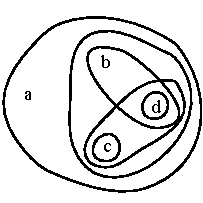
\includegraphics[width=0.3\textwidth]{example-topology.pdf}
        \end{center}
        \caption{Odprte množice na končni množici $X$ iz primera \ref{ex1}}
    \end{figure}
    \begin{figure}[h]
        \begin{center}
        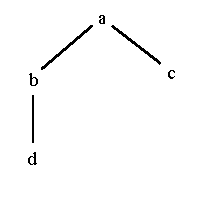
\includegraphics[width=0.3\textwidth]{hasse-example.pdf}
        \end{center}
        \caption{Hassejev diagram končne delno urejene množice iz primera \ref{ex1}}
        \label{pic2}
    \end{figure}
    Ker je množica delno urejena, lahko prostor predstavimo lepše z Hassejevim diagramom (Slika \ref{pic2}).
    To lahko naredimo za vse končne $T_0$ prostore. Hassejev diagram je graf,
    kjer so vozlišča elementi množice, povezave pa urejeni pari $(x,y)$, kjer je $x < y$ in
    ne obstaja $z \in X$, da bi veljalo $x < z < y$. Namesto puščic na povezavah
    predstavimo elemente višje v diagramu. Torej če je $x < y$, potem je $y$
    narisan nad $x$.

\end{example}
Na delni urejenosti lahko definiramo nekaj izrazov. Element $x$ je \textbf{maksimalen},
če $y \geq x$ implicira $y=x$ in je \textbf{maksimum} delne urejenosti, če velja
$y \leq x$ za vsak $y \in X$. Delna urejenost ima \textbf{maksimum}, če in samo če
obstaja natanko en maksimalen element. \textbf{Minimalen} element in \textbf{minimum} sta
definirana dualno.\\
\textbf{Veriga} v delni urejenosti je podmnožica elementov, ki so paroma primerljivi.
\textbf{Antiveriga} je podmnožica elementov, ki so paroma neprimerljivi.\\

%% flag complex
\section{Simplicialni kompleksi}
Simplicialni kompleks $K$ je sestavljen iz množice $V_K$ in množice $S_K$, ki je
sestavljena iz končnih, nepraznih podmnožic množice $V_K$.
$V_K$ se imenuje množica točk, $S_K$ pa množica simpleksov. Veljati mora, da
je vsaka podmnožica moči 1 množice $V_K$ simpleks in vsaka neprazna podmnožica
simpleksov je simpleks. Lahko malenkost izrabimo notacijo in pišemo $v \in K$ namesto
$v \in V_K$ in $\sigma \in K$ namesto $\sigma \in S_K$. V večini primerov bomo
simplicialni kompleks identificirali samo kot množico njegovih simpleksov.\\
Če je simpleks $\sigma$ podmnožica simpleksa $\tau$, pravimo, da je $\sigma$ njegovo \textbf{lice}.
Simpleks, ki ima $n+1$ točk, imenujemo \textbf{$n$-simpleks} in pravimo, da je \textbf{dimenzije} $n$.
Torej vse točke $K$ predstavljajo 0-simplekse. Dimenzija $K$ je supremum dimenzij
vseh simpleksov v $K$. Če je $K$ prazen, ima dimenzijo -1, če ima $K$ simplekse
poljubno velike dimenzije, je dimenzije neskončno.\\
Naj bo $\sigma = \{v_0,v_1,\dots,v_n\}$ simpleks dimenzije $n$. Zaprt simpleks
$\bar{\sigma}$ je množica konveksnih kombinacij točk v $\sigma$.
\[
  \bar{\sigma} = \left\{\sum_{i=0}^n \lambda_i v_i | \lambda_i \geq 0, \sum_{i=0}^n \lambda_i = 1\right\}
\]
Geometrijska realizacija $|K|$ simplicialnega kompleksa $K$ je množica 
vseh takih konveksnih kombinacij $\sum_{v\in K} \lambda_v v,\ \lambda_v \geq 0$, tako da vsi $v$, ki imajo
neničelno $\lambda_v$ tvorijo simpleks v $K$. $|K|$ je torej unija vseh zaprtih
simpleksov $K$.
\begin{example}
  Naj bo $K$ simplicialni kompleks, ki vsebuje simplekse
  $\{a,b,c\}$, $\{b,d\}$, $\{c,d\}$, $\{b,e\}$, $\{f\}$ in vse njihove neprazne
  podmnožice.
  Geometrijska realizacija $|K|$ je prikazana na sliki \ref{sx}.
  \begin{figure}[h]
      \begin{center}
      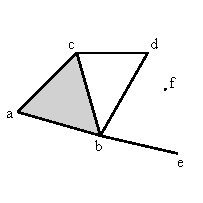
\includegraphics[width=0.4\textwidth]{simplicialni-kompleks.pdf}
      \end{center}
      \caption{Geometrijska realizacija simplicialnega kompleksa $K$}
      \label{sx}
  \end{figure}
\end{example}
\newpage
Topološki prostor $X$ je \textbf{topološki polieder},če obstaja simplicialni
kompleks $K$, da je $X$ homeomorfen telesu $|K|$. Simplicialni kompleks
$K$ imenujemo \textbf{triangulacija} poliedra $X$.
\begin{example}
  Pokažemo lahko, da je kolobar topološki polieder tako, da skiciramo njegovo
  triangulacijo.
    \begin{figure}[h]
        \begin{center}
        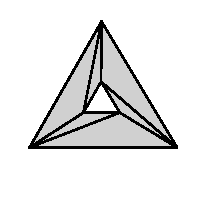
\includegraphics[width=0.4\textwidth]{torus-simpleks.pdf}
        \end{center}
        \caption{Triangulacija kolobarja}
    \end{figure}
\end{example}
Za dan simplicialni kompleks $K$, lahko konstruiramo njegovo \textbf{baricentrično subdivizijo} $K'$.
Točke $K'$ so simpleksi $K$ in simpleksi $K'$ verige simpleksov $K$. Veriga
simpleksov je taka množica $\{\sigma_0,\sigma_1,\dots,\sigma_n\}, \sigma_i \in K$
, da velja $\sigma_0 \subsetneq \sigma_1 \subsetneq \dots \subsetneq \sigma_n$.
\newpage
\begin{figure}[h]
  \begin{center}
  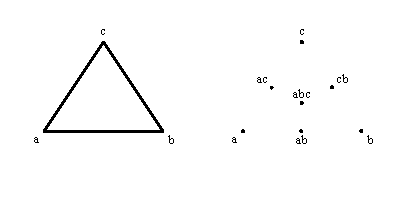
\includegraphics[width=0.8\textwidth]{baricentricna1.pdf}
  \end{center}
  \caption{Prvi korak baricentrične subdivizije}
  \label{baricent1}
\end{figure}
\begin{figure}[h]
  \begin{center}
  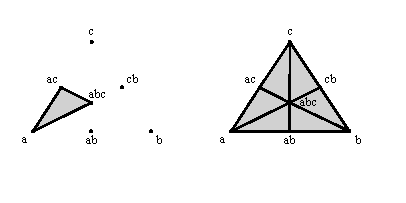
\includegraphics[width=0.8\textwidth]{baricentricna2.pdf}
  \end{center}
  \caption{Simpleks $\{a, ac, abc\}$ in rezultat baricentrične subdivizije}
  \label{baricent2}
\end{figure}
\begin{example}
  Naj bo $K$ 2-simpleks $\{a,b,c\}$. Če hočemo konstruirati baricentrično subdivizijo $K$,
  moramo najprej dodati točke za vsak simpleks v $K$ (Slika \ref{baricent1}).
  Nato dorišemo še najdaljše verige, saj so v tem primeru vsi ostali simpleksi v $K'$ podmnožice teh.
  Primer take verige je $\{a, ac, abc\}$, saj velja $a \subsetneq ac \subsetneq abc$ (Slika \ref{baricent2}).
\end{example}

\section{Povezava delnih urejenosti in simplicialnih kompleksov}
\begin{definition}
  Naj bo $X$ končni $T_0$ topološki prostor. Simplicialni kompleks $\mathcal{K}(X)$
  asociran z $X$ je simplicialni kompleks, katerega množica simpleksov so neprazne verige $X$.
\end{definition}
\begin{definition}
  Naj bo $K$ simplicialni kompleks. Asocirana Delna urejenost $\mathcal{X}(K)$ je
  množica simpleksov $K$ urejeni z inkluzijo. Če sta $\sigma, \tau \in K$,
  je $\sigma \leq \tau$, če je $\sigma \subseteq \tau$.
\end{definition}

\chapter{Digitalni prostori}
Glavni cilj digitalne topologije in digitalne geometrije je premostiti vrzel
med geometrijskimi in topološkimi lastnosti komputacijskih objektov in njihovimi
teoretičnimi reprezentacijami v zveznem prostoru $R^n$. Če hočemo uporabiti
topološke pojme v digitalni domeni, moramo najprej definirati prostor, ki je
analogen zveznemu prostoru $R^n, (n > 1)$.\\
Navadno definiramo digitalne prostore na dva načina. Lahko se odločimo katero 
vrsto povezanosti ima prostor. Naj bo $x = (x_1,\dots,x_n)$
točka v $\mathbb{Z}^n$.\\
  ($3^n-1$)-sosed točke $x$ je vsaka točka
  $y = (y_1,\dots,y_n) \in \mathbb{Z}^n$, za katero velja
  \[
    \max|x_i - y_i| = 1
  \]
  Na primer $n = 2$ nam porodi 8-povezano mrežo.\\
  $2n$-sosed točke $x$ je vsaka točka $y = (y_1,\dots,y_n) \in \mathbb{Z}^n$,
  za katero velja
  \[
    \sum_{i=1}^{n}|x_i - y_i| = 1
  \]
  Na primer $n = 2$ nam porodi 4-povezano mrežo.\\
  V oddelku \ref{obstoj} bomo pokazali, da 8-povezana mreža nima kompatibilne topologije.
\section{Celični kompleksi}
\begin{quote}
    TODO: Laična razlaga celičnih kompleksov in njihove uporabe
\end{quote}

\section{Topologije na grafih}
\begin{definition}
  Za dan topološki prostor $(X, \tau)$ in dano podmnožico $S \subseteq X$, definiramo
  topologijo, zožano na $S$ \[\tau|_S = \{U \cap S\ |\ U \in \tau\}\]
\end{definition}
\begin{definition}
  Naj bo $G = (V,E)$ graf. Naj bo $O$ topologija na $V$. $O$ imenujemo kompatibilna
  topologija na $G$, če velja:
  \begin{itemize}
    \item[(1)] Za vsak povezan $G' \sqsubseteq G$ je $V(G')$ povezan v $O$.
    \item[(2)] Za vsako podmnožico $V' \subseteq V$, ki je povezana v $O$, je $G[V']$ povezan graf.
  \end{itemize}
\end{definition}
\begin{theorem}\label{theorem1}
  Naj bo $G$ graf s kompatibilno topologijo $O$. Za vsak induciran podgraf
  $H \sqsubseteq G$ je topologija, omejena na $V(H)$, kompatibilna topologija
  na grafu $H$. Tako topologijo označimo z $O|_{V(H)}$.
\end{theorem}
\begin{proof}
  Za vsak $H' \sqsubseteq H$ imamo $O|_{V(H')} = O|_{V(H)}|_{V(H')}$. Množica $V(H)$
  je podmnožica $V(G)$, zato je $O|_{V(H)}$ podmnožica $O$.
  Torej vsaka
  podmnožica $V(H)$ je povezana v $O|_{V(H)}$, če in samo če je povezana v $O$.
  $H' \sqsubseteq G$ je povezan, če in samo če je $V(H') \subseteq V(H)$ povezan v $O$.\\
\end{proof}

\section{Topologija dvodelnih grafov}
Naj bo $G^b$ povezan dvodelen graf $G^b = (V,E)$, ki ima vsaj tri vozlišča.
$V$ je torej unija dveh nepraznih disjunktnih množic $V_A$ in $V_B$. Vsaka
povezava v $E$ povezuje samo vozlišča iz $V_A$ z vozlišči iz $V_B$.\\
Definiramo dve kompatibilni topologiji na množici vozlišč $V$ tako, da opišemo
topološko okolico vsake točke $x \in V$. To je najmanjša odprta množica, ki
vsebuje $x$: $U_x \in O$. Ker $U_x$ ni mogoče razdeliti na odprte množice, je $U_x$
in vsaka podmnožica $U_x$, ki vsebuje $x$ povezana.
Poleg tega, je vsaka $U \in O, U \neq \emptyset$ unija določenih $U_x$.\\
Naj bo $N_x = \{y \  | \  yx \in E\}$ množica sosednjih točk točke $x$.\\
\[
  \begin{split}
  O_1:&\quad
  U_x:=\{x\}\ \ \forall x \in V_A, \quad
  U_x:=\{x\}\cup N_x\ \  \forall x \in V_B\\
  O_2:&\quad
  U_x:=\{x\}\cup N_x\ \  \forall x \in V_A, \quad
  U_x:=\{x\}\ \ \forall x \in V_B\\
\end{split}
\]
Kompatibilni topologiji $O_1$ in $O_2$ nista ekvivalentni, razen na grafih,
ki nimajo povezav; lahko nista niti homeomorfni.
\begin{theorem}
  $O_1$ in $O_2$ sta kompatibilni topologiji na $G^b$.
\end{theorem}
\begin{proof}
  Naj bo $O$ enak $O_1$ ali $O_2$.
  \begin{itemize}
    \item[(1)] Naj bo $G' \sqsubseteq G^b$ povezan graf. Dokazati želimo, da je
    množica $V(G')$ povezana v $O$, torej, da je ne moremo razdeliti na dve
    disjunktni odprti podmnožici. Za vsaki dve sosednji točki $x$ in $y$ je
    $U_x \cap U_y$ zmeraj neprazen, saj $y \in U_x$ ali $x \in U_y$. $V(G')$
    razdelimo na dve neprazni disjunktni množici $V_1$ in $V_2$,
    $V(G') = V_1 \cup V_2$. Naj bo $A \in O|_{V(G')}$
    najmanjša odprta množica, ki vsebuje $V_1$, in $B \in O|_{V(G')}$
    najmanjša odprta množica, ki vsebuje $V_2$. Tedaj je $A \cap B \neq \emptyset$,
    torej je $V(G')$ povezan v $O$.
    \item[(2)] Naj bo $G' \sqsubseteq G^b$ nepovezan graf. Dokazati želimo, da
    je množica $V(G')$ nepovezana v $O$. Ker je $G'$ nepovezan, lahko $G'$ razdelimo
    na unijo dveh ne nujno povezanih induciranih podgrafov $C$ in $D$ tako, da nobeno vozlišče iz $C$
    ni povezano z nobenim vozliščem iz $D$. Torej
    \[\bigcup_{x\in V(C)}U_x \cap V(D) = \emptyset = V(C) \cap \bigcup_{x\in V(D)}U_x\]
    $V(C)$ in $V(D)$ lahko razpišemo:
    \[V(C) = V(G') \cap \left(\bigcup_{x\in V(C)} U_x\right)\]
    \[V(D) = V(G') \cap \left(\bigcup_{x\in V(D)} U_x\right)\]
    Vidimo, da sta $V(C)$ in $V(D)$ disjunktni odprti množici v $O|_{V(G')}$,
    torej je $V(G')$ nepovezana v $O$.
  \end{itemize}
\end{proof}

Naj bo $O$ poljubna kompatibilna topologija na $G^b$. Naslednje leme držijo za $\forall x \in V$
\begin{lemma}\label{lem1}
  $\{x\} \subseteq U_x \subseteq \{x\} \cup N_x$
\end{lemma}
\begin{proof}
  $\{x\} \subseteq U_x$ sledi iz definicije. Recimo, da obstaja $x'$, da
  $U_{x'} \nsubseteq \{x'\} \cup N_{x'}$ ne drži, potem obstaja
  $y \in U_{x'}$, $y \notin (\{x'\} \cup N_{x'})$. Ker je $\{x', y\} \subseteq U_x$,
  je ta množica povezana v $O$. Ker je $G^b[\{x',y\}]$ nepovezan graf, je to v
  protislovju z definicijo kompatibilne topologije na $G^b$.
\end{proof}
\begin{lemma}\label{lem2}
  $U_x = \{x\}$ ali $U_x = \{x\} \cup N_x$
\end{lemma}
\begin{proof}
  Recimo, da lema ne drži. Potem obstaja $x'$, da $U_{x'} \neq \{x'\}$ in
  $U_{x'} \subsetneq \{x'\} \cup N_{x'}$. Torej obstaja $y \in N_{x'}$, $y \notin U_{x'}$.
  Ker je $y \in N_{x'}$, sta $x$ in $y$ povezana. Ker sta povezana in je $G^b$
  dvodelen graf, velja $N_{x'} \cup N_y = \emptyset$. Ker sta $U_{x'}$ in $U_y$ 
  podmnožici $N_x'$ in $N_y$, je bodisi $U_{x'} \cap U_y = \emptyset$,
  bodisi $U_{x'} \cap U_y = \{x'\}$. Če velja $U_{x'} \cap U_y = \emptyset$, sledi
  protislovja, ker $\{x',y\}$ je povezana množica v $O$.
  Če velja $U_{x'} \cap U_y = \{x'\}$, potem je $U_{x'} = \{x'\}$, kar je v
  protislovju z predpostavko $U_{x'} \neq \{x'\}$.
\end{proof}
\begin{lemma}\label{lem3}
  Za vsak $y \in N_x$ velja $U_x = \{x\} \iff U_y = \{y\} \cup N_y$
\end{lemma}
\begin{proof}
Če je $U_x = \{x\}, U_y = \{y\}$ za katerikoli $y$, sledi protislovje, saj je 
$\{x,y\}$ nepovezana v $O$, $y$ pa je sosed $x$.
Če velja $U_x = \{x\} \cup N_x, U_y = \{y\} \cup N_y$ za katerikoli $y$, potem je
$U_x \cap U_y = \{x, y\} \in O$ (ker je $y \in N_x \Rightarrow x \in N_y$). Ker je
$U_x$ najmanjša odprta množica, ki vsebuje $x$, je $U_x = \{x,y\}$. Prav tako je
tudi $U_y = \{x,y\}$. Zaradi leme \ref*{lem2}, sledi, da je $N_x = \{y\}$ in $N_y = \{x\}$.
Ker je graf povezan in je edini sosed $x$ $y$, sta ti dve točki cel graf
$V(G^b) = \{x,y\}$, kar je protislovje s predpostavko, da ima $G^b$ vsaj tri vozlišča.
\end{proof}

Iz zadnje leme sledi:
\begin{theorem}
Vsak povezan, dvodelen graf $G^b = (V,E)$, ki ima vsaj tri vozlišča, ima natanko
dve kompatibilni topologiji. To sta $O_1$ in $O_2$:
\[
  \begin{split}
  O_1:&\quad
  U_x:=\{x\}\ \ \forall x \in V_A, \quad
  U_x:=\{x\}\cup N_x\ \  \forall x \in V_B\\
  O_2:&\quad
  U_x:=\{x\}\cup N_x\ \  \forall x \in V_A, \quad
  U_x:=\{x\}\ \ \forall x \in V_B\\
\end{split}
\]
\end{theorem}

\section{Obstoj kompatibilne topologije na grafu} \label{obstoj}

\begin{corollary}\label{corollary1}
Krog $C$, ki ima sodo število vozlišč $n > 3$, nima kompatibilne topologije.
\end{corollary}
\begin{proof}
Za vsak $x \in V(C), G_x^b := C[\{x\} \cup N_x]$ je dvodelen graf, ki ima vsaj tri
vozlišča. Recimo, da ima $C$ kompatibilno topologijo $O$ na vsakem $G_x^b$ je inducirana 
kompatibilna topologija $O_1$ ali $O_2$. Za vsaki dve sosednji točki $x,y \in V(C)$ velja:
\[
    O|_{V(G_x^b)} \cong O_1 \iff O|_{V(G_y^b)} \cong O_2
\]
sicer, bi $U_x = \{x\}$ in $U_y = \{y\}$, kar bi pomenilo, da je množica
$\{x, y\}$ nepovezana v $O$ in to je v protislovju z predpostavko, da sta $x$ in
$y$ povezana. Če si izberemo neko začetno točko $X_0 \in V(C)$, lahko zaporedno
izbiramo sosednje točke in opazujemo inducirane kompatibilne topologije.
\[O|_{V(G_{X_0}^b)} \cong O_1\]
\[O|_{V(G_{X_1}^b)} \cong O_2\]
\[O|_{V(G_{X_3}^b)} \cong O_1\]
Ker ima krog sodo število vozlišč, se na $x_0$ inducira kompatibilna topologija $O_2$. Torej
na podgraf $G^b_{x_0}$ sta inducirani kompatibilni topologiji $O_1$ in $O_2$, kar je v protislovju.
\end{proof}

Iz posledice \ref*{corollary1} in iz Izreka \ref*{theorem1} sledi:
\begin{theorem}
Vsak graf $G$, ki vsebuje krog $C$ s lihim številom vozlišč, kot induciran podgraf,
nima kompatibilne topologije.
\end{theorem}
Zaradi izreka lahko sklepamo, da 8-povezana mreža nima kompatibilne topologije,
saj vsebuje krog s lihim številom vozlišč kot induciran podgraf (Slika \ref{oddCircle}).
\begin{figure}
  \begin{center}
  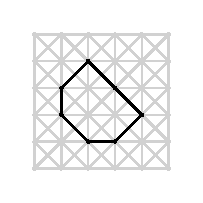
\includegraphics[width=0.4\textwidth]{odd_circle.pdf}
  \end{center}
  \caption{krog s lihim številom vozlišč kot induciran podgraf 8-povezane mreže}
  \label{oddCircle}
\end{figure}

\nocite{*}
\cleardoublepage
\addcontentsline{toc}{chapter}{Literatura}
\bibliography{literatura}
\bibliographystyle{plainnat}

\end{document}

